\section{Parameterized Quantum Circuit Based Localization}
\label{sec:pqc-loc}


\begin{figure*}
    \centering
    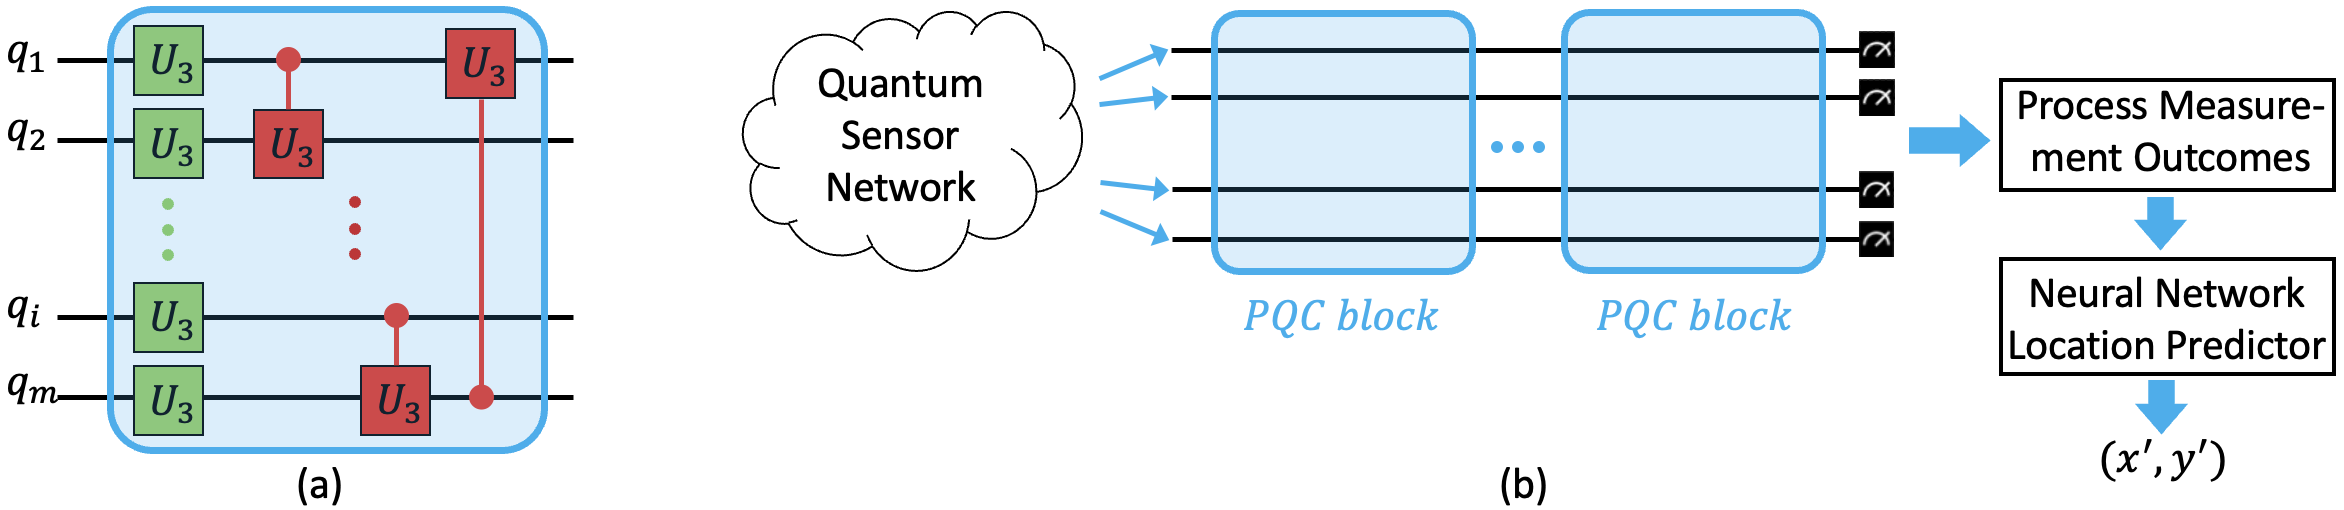
\includegraphics[width=0.99\textwidth]{chapters/qce/figures/pqc.png}
    \caption{(a) Our parameterized quantum circuit (PQC) block, for the general case of $m$ qubits. It contains $m$ number of $U_3$ gates and $m$ number of $CU_3$ gates.
    (b) The hybrid quantum-classical circuit to localize a transmitter. It consists of multiple PQC blocks, followed by classical processing of measurements, and finally, a neural network-based location predictor. We use only four blocks of PQCs in our hybrid circuit.
    }
    \label{fig:pqc}
\end{figure*}

\para{Motivation.} The QSD-based method discussed in the previous section has a solid mathematical foundation, but its practical implementation is non-trivial and even infeasible for a large sensor network and/or a large number of potential transmitter locations. 
%%%%%%%%%%%%%%%%%%
In particular, the POVM measurement operator (derived from the QSD problem or corresponding to the pretty-good measurement)
can be infeasible to implement for a 
large number of outcomes/locations. 
%%%%%%%%%%%%%%%%%%
The issue is somewhat mitigated by using a two-level approach as described above, but the PoE (probability of error) 
in the first (coarser) level can still be high due to imperfect training (as we assign a single outcome to a {\em set} of
target locations). 
%%%%%%%%%%%%%%%%%%%%%%%%%%
A potential approach to address the above challenge is to ``translate'' a given POVM into an appropriate quantum circuit comprised of quantum gates and simple
measurements (e.g., projective and/or computational basis)~\cite{pra19-povm}. E.g.,~\cite{qcompiler} presents a technique to convert POVM operators to such quantum circuits. 
%%%%%%%%%%%%%%%%%%%%%%%%%%
However, the computational time incurred in translating a POVM operator into a quantum circuit 
is exponential to the number of qubits and is thus infeasible. In addition, the translated quantum circuits 
are also sub-optimal in terms of the number of CNOT gates used~\cite{qcompiler}.
Also, note that the POVM computed in our QSD-based method is sub-optimal to begin with.
%%%%%%%%%%%%%%%%%%%%%%%%%%%%%%%

In this section, we develop a machine learning (ML) technique to actually learn a quantum circuit that represents the processing and measurement protocol needed to localize the transmitter from the evolved quantum state.
% \red{The quantum circuits are optimized by a classical computer through the hybrid quantum-classical paradigm.}
The learned quantum circuit model maps the global evolved quantum state to the transmitter location.
%%%%%%%%%%%%%%%%%
In essence, we avoid computing the POVM (from QSD, or using the pretty-good measurement) altogether (and thus, also avoid the challenge of translating it to a quantum circuit), and instead learn the required quantum circuit representing the measurement protocol.
%%%%%%%%%%%%%%%%%%%%%%
To facilitate learning the quantum circuit, we use an appropriate parameterized quantum circuit (PQC) and learn 
its parameters---as in~\cite{PhysRevResearch.qsd-qnn} 
wherein a POVM is trained using parameterized quantum circuits.
%%%%%%%%%%%%%%%%%%%%%%%%%%%
Our PQC-based localization method based on the above insights is described
below. We start with a brief introduction to PQCs.

\para{Parameterized Quantum Circuits (PQC)}.
Parameterized quantum circuits have emerged as a powerful tool in quantum computing~\cite{Benedetti_2019}, providing an adaptable framework for tackling diverse computational tasks. 
Parameterized quantum circuits (PQCs) can be regarded as machine learning models with remarkable expressive power; just like classical ML models, PQC circuits/models are trained to perform data-driven tasks. 
%%%%%%%%%%%%%%%%%%%%%%%%
PQCs offer several advantages over fixed quantum circuits~\cite{Benedetti_2019, quantumnas2022,quantumnat2022}, including:
\begin{enumerate}
    \item Adaptability. The parameters in PQCs can be adjusted to tailor the circuit for a specific problem, allowing a single circuit structure to be repurposed for various tasks.
    \item Trainability. PQCs can be trained using classical optimization algorithms to solve optimization problems and machine learning tasks, making them a vital component of hybrid quantum-classical algorithms. 
    \item Noise Resilience. PQCs can be more robust against noise and errors in near-term quantum devices, as they allow shorter-depth circuits that reduce the impact of errors. 
\end{enumerate}

In essence, PQCs are quantum circuits comprised of parameterized gates and measurements.
Commonly used parameterized gates in PQCs include rotation gates $R_x(\theta),$ $R_y(\theta),R_z(\theta)$ which represents rotating about the $X,Y,Z$ axis respectively with angle $\theta$.
A more versatile gate is the $U_3(\theta, \phi, \lambda)$, which can be used to generate any single-qubit operation by setting the appropriate values for the parameters;
$U_3$ gate can be decomposed into simpler $R_x, R_y, R_z$ gates.
The parameterized $CU_3(\theta, \phi, \lambda)$ gate is the controlled 
version of the $U_3$ gate; it applies the $U_3$ gate only when the control qubit 
is in the $\ket{1}$ state.
We use a combination of $U_3$ and $CU_3$ gates in our parameterized quantum circuits. 

\para{PQC-based Localization Method}.
At a high level, in our PQC-based localization scheme, the QSN data is fed into a trained hybrid quantum-classical model, which represents the overall measurement strategy and thus outputs the transmitter location. 
%%%%%%%%%%%%%%
Our hybrid quantum-classical model (see Fig.~\ref{fig:pqc}(b)) consists
of the following three components.
%%%%%%%%%%%%%
(i) Parameterized Quantum Circuit (PQC), (ii) Processing the measurement outcomes,
(iii) Neural network location predictor, to convert the processed measurement outcomes to the transmitter location.
We describe each of the above components below.

\softpara{1. Parameterized Quantum Circuit (PQC) Design.}
The parameterized quantum circuit can be designed in many ways. 
We design our PQC component based on some common PQC-design patterns~\cite{liang2023unleashing, ICCAD21-wang} used in prior works.
For example, in~\cite{lloyd2020quantum}, a block of 
PQC contains one layer of $ZZ$ gates 
and one layer of $R_y$ gates.
In~\cite{McClean_2018}, a block of PQC contains one layer each
of $R_x, R_y, R_z, CZ$ gates.
In our scheme, the quantum circuit is composed of blocks, and 
each block is a combination of $U_3, CU_3$ gates;
we use these two gates in our design as they form a universal
gate set and are widely used in PQC circuits.
Circuits consisting $U_3$ and $CU_3$ gates have a high expressive power as each gate has three trainable parameters.
%%%%%%%%%%%%%%%%%%%%
% We pick these two gates because they are called the ``swiss army knife'' of parameterized quantum gates.
%%%%%%%%%%%%%%%%%%%%%%%%%%
In particular, given $N$ number of input qubits, a block consists of 
$N$ number of $U_3$ and $N$ number of $CU_3$ gates. 
See Fig.~\ref{fig:pqc}.
%%%%%%%%%%%%%%%%%%%%
In a block, each input qubit is first  
operated on by the unary $U_3$ gate in parallel,
forming a layer of $U_3$ gates. 
Then, there is a series of $CU_3$ gates following a ring connection pattern, 
i.e., each $CU_3$ is executed over two ``consecutive'' qubits (with the first being
the control qubit) except for the
last $CU_3$ gate which is over the last and the first qubit. 
%%%%%%%%%%%%%%%%%%%%%%%%%%%%%
Thus, a single block has a circuit depth of $N+1$.
The overall PQC may have a series of above blocks---the expressive power of the model increases monotonically with the increase in the number of blocks.
%%%%%%%%%%%%%%%%%%%%
In our evaluations (\S\ref{sec:eval}), we used four blocks as we observed that four blocks provide good performance while having a modest circuit depth.
%%%%%%%%%%
After the blocks, the PQC ends with the measurement on the standard computational basis, 
i.e., the Pauli Z basis.

\softpara{2. Process Measurement Outcomes.} 
As in the QSD-based schemes, we will use the PQC to make repeated measurements.
To use the repeated measurements effectively for location prediction, we characterize
the set of repeated measurement results by expectation values, one for each qubit.
%%%%%%%%%%%%%%%%%
In particular, we compute the expectation value 
$\langle Z \rangle$ of the Pauli Z operator 
(which represents
the measurement in the computational basis), and feed as input to a neural network for 
final location prediction as described below. 
We note that, for a quantum state $\ket{\psi} = \alpha \ket{0} + \beta \ket{1}$, the expectation value 
$\langle Z \rangle$ of the Pauli Z operator is given by $\bra{\psi} Z \ket{\psi} = |\alpha|^{2} - |\beta|^{2}$.



% For $\ket{\psi} = \alpha \ket{0} + \beta \ket{1}$, $\langle Z \rangle = |\alpha|^{2} - |\beta|^{2}$ is the measure of how much the probabilities are biased towards $\ket{0}$ and $\ket{1}$.
% The expectation values of the measurement operators are fed into a neural network for final location prediction as described next. 

\softpara{3. Neural Network to Predict Location.}
We consider two variants of our neural network predictor: (i) Classifier variant. which outputs a class/label corresponding to the cell where the TX is located, and thus, predicts the location to be the cell's center. (ii) 
Regression variant, that outputs locations as the $x$ and $y$ coordinates.

{\em Classifier Variant.}
In~\cite{jindi2023}, a novel quantum label-based supervised learning approach is proposed to perform multi-classification.
Our overall circuit with the Classifier component for the location prediction essentially equates to a circuit for quantum state discrimination (QSD), as the 
QSD problem also outputs a finite number of discrete outcomes.
%%%%%%%%%%%%%%%%%
For the Classifier Variant, we use a simple neural network with only an input layer and an output later, having no hidden layers---i.e., a single 
fully connected layer.
%%%%%%%%%%%%%%%%
The input neurons are the expectation values of the Pauli Z operator from the measurements as described above, and the output neurons represent the cell labels. See Fig.\ref{fig:fclayer}(a), which shows the fully connected layer for a network of 4 quantum sensors deployed in a $4\times 4$ grid with 16 cells.

{\em Regression Variant.}
The Classifier Variant outputs locations in a discrete space---which is fundamentally sub-optimal if the transmitter can be anywhere in the 2D space. 
%%%%%%%%%%%%%%%%%%%%
To output the predicted location in the continuous 2D space, we use a Regression Variant that outputs the location as an $(x,y)$ point.
For the setting wherein the transmitter may be located anywhere in the 
2D space, the Regression Variant should have a smaller localization error.
Fig.\ref{fig:fclayer}(b) shows the fully connected layer for the Regression Variant; the number of output neurons is always two, i.e., a $X$ coordinate and a $Y$ coordinate.

\softpara{4. Loss Function.}
% The loss function quantifies the difference between the predicted location and the ground truth location. 
During training, the gradient of the loss function is back-propagated through the neural network and the quantum circuit parts, so that the parameters within these parts can be appropriately updated. 
The loss functions used for the Classifier Variant and the Regression Variant are different; for the Classifier variant, we use the cross-entropy loss function while for the Regression variant, we use the mean square error loss function.

% It is not hard to realize that a simple change in the fully connected layer's output neurons will turn the classification solution into a regression solution.
% The benefit of modeling a localization problem as a regression problem is that the solution directly outputs the location in the continuous space.
% Since the transmitter locations, in general, are in the continuous space, a regression representation will have a smaller localization error.

\para{\pqcone and \pqctwo Schemes.} 
The above-described hybrid quantum-classical model is essentially our \pqcone localization scheme.
By using \pqcone as a building block and using the same two-level (coarse, fine) idea described in~\S\ref{sec:povm}, we design the \pqctwo, corresponding to the two-level QSD-based schemes described in the previous section.
At the first coarse level, the output of the ``coarse-level \pqcone'' will determine the block the transmitter is in.
Then at the second fine level, the output of the ``fine-level \pqcone'' tied to the block determined by the coarse level is the final location output.
The PQC-based schemes essentially use the trained circuit in lieu of the POVM used in the QSD-based schemes. 
%%%%%%%%%%%%%%%%%%%%
The PQC-based schemes can be used with either the Classifier or the Regression variant
for the last predictor component. 




\begin{figure}
    \centering
    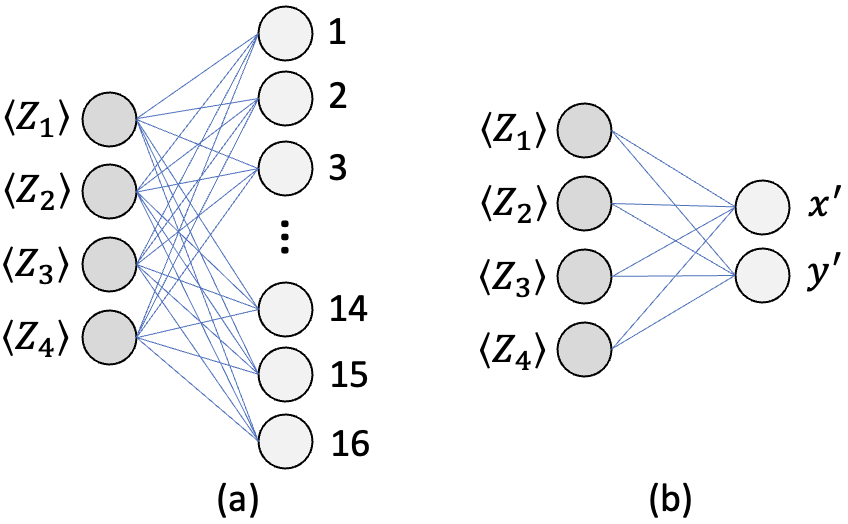
\includegraphics[width=0.5\textwidth]{chapters/qce/figures/fclayer.png}
    \caption{Neural network (a fully connected layer) for 4 quantum sensors to predict the location from processed measurements. (a) Classifier Variant, (b) Regression Variant.}
    \label{fig:fclayer}
\end{figure}

% Motivation for parameterized quantum circuit 
% \begin{enumerate}
%     \item Computing the optimal POVM is intractable. Semidefinite programming is too slow when larger than 5 qubits.
%     \item PGM heuristic is an option but is also hard to implement \cite{...}.
%     \item Better accuracy.
%     \item Easy to evaluate (memory and time). Able to implement on a real quantum computer.
% \end{enumerate}



